\documentclass{article}

\usepackage{amsmath}
\usepackage{amssymb}
\usepackage{amsfonts}
\usepackage{fullpage}
\usepackage{graphicx}
\usepackage{float}


\makeatletter
\def\moverlay{\mathpalette\mov@rlay}
\def\mov@rlay#1#2{\leavevmode\vtop{%
   \baselineskip\z@skip \lineskiplimit-\maxdimen
   \ialign{\hfil$\m@th#1##$\hfil\cr#2\crcr}}}
\newcommand{\charfusion}[3][\mathord]{
    #1{\ifx#1\mathop\vphantom{#2}\fi
        \mathpalette\mov@rlay{#2\cr#3}
      }
    \ifx#1\mathop\expandafter\displaylimits\fi}
\makeatother

\newcommand{\cupdot}{\charfusion[\mathbin]{\cup}{\cdot}}
\newcommand{\bigcupdot}{\charfusion[\mathop]{\bigcup}{\cdot}}

\title{MA 2631 Assignment 2}
\author{Hubert J. Farnsworth}

\setlength\parindent{0pt}
\begin{document}
\maketitle

\begin{enumerate}

%%%% 1 %%%%

\item

65 students are registered for a math class, which will be held in two sections.

\begin{enumerate}
\item In how many ways can the students be split into two sections?

\item Due to the size of the classroom at most 34 students can be in each section. In how
many ways can the two sections be organized under this constraint?
\end{enumerate}

Answer:

\begin{enumerate}
\item For each of the 65 students, there are 2 choices for which class the student can be assigned to. This gives $2^{65}$ ways. Exclude the 2 cases in which all students are assigned to the same class, leaving the other empty. Therefore there are $2^{65} - 2 \approx 3.7 \cdot 10^{19}$ ways to split the students into two sections. 

\item Since each section can accommodate no more than 34 students, the only allowable values for the number of students in a classroom are 34, 33, 32, and 31. 

$$
\binom{65}{34} + \binom{65}{33} + \binom{65}{32} + \binom{65}{31} \approx 1.4 \times 10^{19}.
$$ 

\end{enumerate} 

 
\newpage
%%%% 2 %%%%

\item Prove by induction that for all positive integers n it holds that

$$ \sum_{k=0}^n (-1)^k \binom{n}{k} = 0.$$

Answer: First establish the base case $n=1$.

$$
\sum_{k=0}^1 (-1)^k \binom{n}{k} = (-1)^0 \binom{1}{0} + (-1)^1 \binom{1}{1} = 1 - 1 = 0.
$$

Assume the result holds for $n \geq 1$.

\begin{align*}
\sum_{k=0}^{n+1} (-1)^k \binom{n+1}{k}
&= (-1)^0\binom{n+1}{0} + \sum_{k=1}^{n} (-1)^k \binom{n+1}{k} + (-1)^{n+1}\binom{n+1}{n+1} \\
&= 1 + \sum_{k=1}^{n} (-1)^k \binom{n+1}{k} + (-1)^{n+1} \\
&= 1 + \sum_{k=1}^{n} (-1)^k\left( \binom{n}{k-1} + \binom{n}{k}\right) + (-1)^{n+1} \\
&= 1 + \sum_{k=1}^{n} (-1)^k\binom{n}{k-1} + \sum_{k=1}^n (-1)^k\binom{n}{k} + (-1)^{n+1} \\
&=  \sum_{j=0}^{n-1} (-1)^{j+1}\binom{n}{j} + (-1)^{n+1}  + 1 + \sum_{k=1}^n (-1)^k\binom{n}{k}  \\
&=  \sum_{j=0}^{n-1} (-1)^{j+1}\binom{n}{j} + (-1)^{n+1}\binom{n}{n}  + (-1)^0\binom{n}{0} + \sum_{k=1}^n (-1)^k\binom{n}{k}  \\
&=  -\sum_{j=0}^{n-1} (-1)^{j}\binom{n}{j} - (-1)^{n}\binom{n}{n}  + \sum_{k=0}^n (-1)^k\binom{n}{k}  \\
&= -\sum_{j=0}^{n} (-1)^{j}\binom{n}{j} + \sum_{k=0}^n (-1)^k\binom{n}{k}  \\
&= 0
\end{align*}
 
\newpage
%%%% 3 %%%%

\item There is an easier way to prove this statement of the previous problem, using results
from the lecture. Please provide that proof.

Answer: Using the binomial formula $\sum_{k=0}^n \binom{n}{k} x^{n-k}y^k = (x+y)^n$, 

\begin{align*}
0 &= (1 + (-1))^n \\
&= \sum_{k=0}^n \binom{n}{k}1^{n-k}(-1)^{k} \\
&= \sum_{k=0}^n (-1)^k\binom{n}{k} . 
\end{align*}

\newpage
%%%% 4 %%%%

\item

Let $E, F, G$ be events on a sample space $\Omega$. We know from class the distributive law

$$(E \cup F) \cap G = (E \cap G) \cup (F \cap G). $$

Illustrate by Venn diagrams (one diagram for the left and one for the right hand of the
equation).

\begin{figure}[H]
\centering
  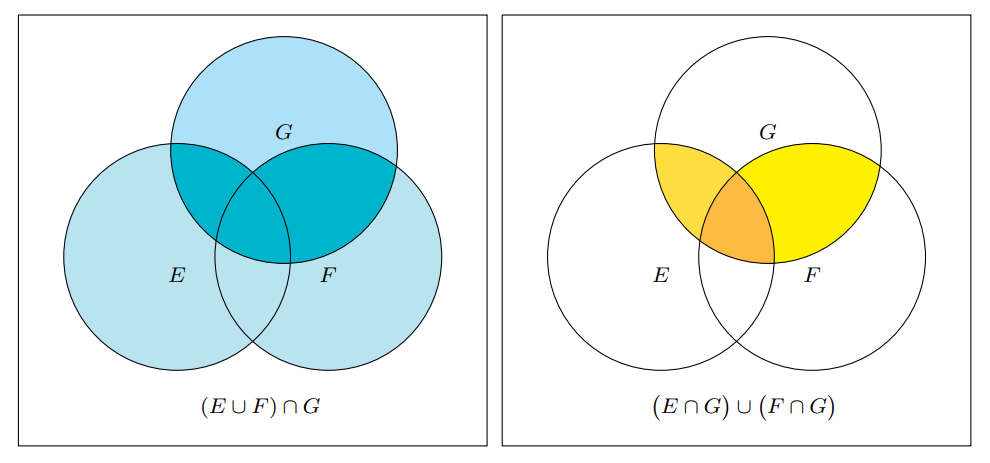
\includegraphics[width=0.65\linewidth]{Capture 1.png}
\end{figure}

\newpage
%%%% 5 %%%%

\item

Given a family of events $E_1, E_2,\dots, E_n, \dots$ on some sample space $\Omega$, construct a new
family $F_1, F_2,\dots ,F_n, \dots$ on the same sample space $\Omega$ such that the $F_i$ are
disjoint and 

$$ \bigcup_{k=1}^n F_k = \bigcup_{k=1}^n E_k. $$

Answer: Define the family $F_n$ by:

\begin{align*}
F_1 &:= E_1 \\
F_2 &:= E_2 \backslash F_1 = E_2 \backslash E_1 = E_2 \cap E_1^c \\
F_3 &:= E_3 \backslash (F_1 \cup F_2 )= E_3 \cap (F_1 \cup F_2)^c = E_3 \cap (F_1^c \cap F_2^c) \\
F_4 &:= E_4 \backslash (F_1 \cup F_2 \cup F_3) =
E_4 \cap (F_1 \cup F_2 \cup F_3)^c = E_4 \cap (F_1^c \cap F_2^c \cap F_3^c) \\
&\vdots \\
F_n &= E_n \backslash \bigcup_{k=1}^{n-1} F_k = E_n \cap \left(\bigcap_{k=1}^{n-1} F_k^c \right).
\end{align*}

To show that the $F_k$ are disjoint, suppose $0<m<n$. 

\begin{align*}
F_n \cap F_m 
&= \left(E_n \cap (\cap_{k=1}^{n-1} E_k^c)\right)
\cap \left(E_m \cap (\cap_{j=1}^{m-1} E_j^c \right) \\
&= \left(E_n \cap (\cap_{k=1}^{m-1} E_k^c) \cap E_m^c \cap (\cap_{k=m+1}^{n-1} E_k^c)\right)
\cap \left(E_m \cap (\cap_{j=1}^{m-1} E_j^c \right) \\
&= \left(E_n \cap (\cap_{k=1}^{m-1} E_k^c) \cap (\cap_{k=m+1}^{n-1} E_k^c)\right)\cap E_m^c \cap E_m \cap 
(\cap_{j=1}^{m-1} E_j^c) \\
&= \left(E_n \cap (\cap_{k=1}^{m-1} E_k^c) \cap (\cap_{k=m+1}^{n-1} E_k^c)\right)\cap \emptyset \cap 
(\cap_{j=1}^{m-1} E_j^c) \\
&= \emptyset.
\end{align*}

Prove that $\bigcup_{k=1}^n F_k  = \bigcup_{k=1}^n E_k$ by induction. For $n = 1$ the equality holds by the definition $F_1 := E_1$. Assume the equality holds for some $n\geq 1$.

\begin{align*}
\bigcup_{k=1}^{n+1} F_k &= F_{n+1} \cup \left(\bigcup_{k=1}^n F_k\right) \\
&= \left( E_{n+1} \cap \left(\bigcup_{k=1}^{n} F_k\right)^c \right)\cup \left(\bigcup_{k=1}^n F_k\right) \\
&= \left( E_{n+1}  \cup \left(\bigcup_{k=1}^{n} F_k\right) \right)\cap \left(\left(\bigcup_{k=1}^{n} F_k\right)^c \cup \left(\bigcup_{k=1}^n F_k\right)\right) \\
&= \left( E_{n+1}  \cup \left(\bigcup_{k=1}^{n} F_k\right) \right)\cap \Omega \\
&= \left( E_{n+1}  \cup \left(\bigcup_{k=1}^{n} F_k\right) \right)\cap \Omega \\
&= \left( E_{n+1}  \cup \left(\bigcup_{k=1}^{n} E_k\right) \right)\cap \Omega \\
&= \left(\bigcup_{k=1}^{n+1} E_k \right)\cap \Omega \\
&= \bigcup_{k=1}^{n+1} E_k.
\end{align*}

\newpage
%%%% 6 %%%%

\item 

4 dice are rolled.

\begin{enumerate}
\item Describe mathematically the sample space of this experiment.

\item Describe mathematically the events

$$ E = \text{”exactly three dice show a six”},$$
$$ F = \text{”at least two dice show a six”}. $$

\item Describe mathematically the events $E^c, E\cap F,  E^c \cup F^c$. 
\end{enumerate}

Answer:

\begin{enumerate}
\item $\Omega = \{(i,j,k,l) : i,j,k,l \in \{1,2,3,4,5,6\}\}$.

\item 
\begin{align*}
E &= \{(6,6,6,k) : k \in \{1,2,3,4,5\}\}
\cup \{(6,6,k,6) : k \in \{1,2,3,4,5\}\} \\
&\cup \{(6,k,6,6) : k \in \{1,2,3,4,5\}\} 
\cup \{(k,6,6,k) : k \in \{1,2,3,4,5\}\}
\end{align*}

\begin{align*}
F &= \{(6,6,k,j) : k,j \in \{1,2,3,4,5,6\} \}
\cup \{(6,k,6,j) : k,j \in \{1,2,3,4,5,6\} \} \\
&\cup\{(6,k,j,6) : k,j \in \{1,2,3,4,5,6\} \}
\cup \{(k,6,6,j) : k,j \in \{1,2,3,4,5,6\} \} \\
&\cup \{(k,j,6,6) : k,j \in \{1,2,3,4,5,6\} \}
\cup \{(k,6,j,6) : k,j \in \{1,2,3,4,5,6\} \}
\end{align*}

\item 

\begin{align*}
E^c &= \{(6,6,6,6)\} \cup \{(i,j,k,l) : i,j,k,l \in \{1,2,3,4,5\}\} \\
&\cup\{(6,6,k,j) : k,j \in \{1,2,3,4,5\} \}
\cup \{(6,k,6,j) : k,j \in \{1,2,3,4,5\} \} \\
&\cup\{(6,k,j,6) : k,j \in \{1,2,3,4,5\} \}
\cup \{(k,6,6,j) : k,j \in \{1,2,3,4,5\} \} \\
&\cup \{(k,j,6,6) : k,j \in \{1,2,3,4,5\} \}
\cup \{(k,6,j,6) : k,j \in \{1,2,3,4,5\} \}\\
&\cup\{(6,i,j,k) : (i,j,k \in \{1,2,3,4,5\}\} 
\cup \{(i,6,j,k) : (i,j,k \in \{1,2,3,4,5\}\} \\
&\cup\{(i,j,6,k) : (i,j,k \in \{1,2,3,4,5\}\} 
\cup \{(i,j,k,6) : (i,j,k \in \{1,2,3,4,5\}\} \\
E\cap F &= E \quad \text{since } E \subseteq F.\\
E^c \cup F^c &= E^c \text{since } F^c \subseteq E^c.
\end{align*}




\end{enumerate}

\end{enumerate}

\end{document}